\documentclass[11pt]{article}

\usepackage[letterpaper,margin=1in]{geometry}
\usepackage[T1]{fontenc}
\usepackage[utf8]{inputenc}
\usepackage{booktabs}
\usepackage{array}
\usepackage{enumitem}
\usepackage{xcolor}
\usepackage{listings}
\usepackage{microtype}
\usepackage{tikz}
\usetikzlibrary{arrows.meta,positioning}
\usepackage[hidelinks]{hyperref}

\definecolor{codebg}{RGB}{247,249,250}
\definecolor{codeframe}{RGB}{220,224,228}
\definecolor{accent}{RGB}{27,94,72}

\emergencystretch=3em

\lstset{
  basicstyle=\ttfamily\small,
  backgroundcolor=\color{codebg},
  frame=single,
  rulecolor=\color{codeframe},
  breaklines=true,
  showstringspaces=false,
  columns=fullflexible,
  keepspaces=true,
  aboveskip=1em,
  belowskip=1em
}

\title{
  \vspace{-2em}
  \textbf{ResonantOS SDK Reference Demo}\\[0.4em]
  \large Technical Report and User Guide\\[0.2em]
  \normalsize \textsc{SDK-DEMO-003}
}

\author{ResonantOS SDK Working Group}
\date{September 25, 2026}

\begin{document}

\maketitle

\begin{abstract}
This report documents \textsc{SDK-DEMO-003}, the reference SDK demonstration
built against the current ResonantOS $2.0.0$-alpha \texttt{dev} line. Three
independently packaged local-service add-ons --- Resonant Echo, Resonant
Counter, and the SDK Guide --- are discovered, validated, registered,
granted, enforced, and revoked through the platform's \emph{existing}
manifest, registry, capability, endpoint-guard, bridge, and extension
mechanisms, with zero add-on-specific Core code and no parallel trust model.
The report describes the objectives, the host-aligned architecture that was
verified, the capability and isolation model, the engineering defects found
and corrected during independent review, the adversarial red-team results, the
test results, a step-by-step user guide, the honest demo-versus-production
boundary, and a concrete way forward toward a production running SDK platform.
\end{abstract}

\tableofcontents

\section{Objectives}

The goal was to move the ResonantOS SDK from a verified contract to a
browser-visible demonstration that \emph{consumes} the platform's real
mechanisms rather than inventing parallel ones. The demonstration had to
answer one question:

\begin{quote}
\itshape
Can a third-party-style add-on be authored against the public
\texttt{@resonantos/addon-sdk} contract, discovered and validated by the host,
registered into the host-owned registry, granted a capability through explicit
operator consent, exercised inside the real browser extension, and revoked ---
returning a real host-policy \texttt{403} --- all through one generic contract,
with no add-on-specific Core code and no second trust model?
\end{quote}

The acceptance criteria were strict:

\begin{itemize}[leftmargin=1.5em]
  \item \textbf{Generic discovery} --- the host scans a canonical location and
        picks up independently packaged add-ons without teaching Core their
        identifiers.
  \item \textbf{Manifest-driven contract} --- identity, version, capabilities,
        and trust posture come from the add-on's own \texttt{addon.json},
        validated by \texttt{validateAddOnManifest}.
  \item \textbf{No self-grant} --- requested capabilities are authored with
        \texttt{granted: false}; grants are minted by the host-owned registry
        only after \texttt{consent: true}.
  \item \textbf{Isolation} --- the add-on UI runs in a sandboxed cross-origin
        iframe and cannot reach extension internals.
  \item \textbf{Real enforcement} --- an authorized call returns \texttt{200},
        a wrong credential returns \texttt{401}, and a revoked grant returns
        \texttt{403} from the upstream, not a renderer-side simulation.
  \item \textbf{Replacement proof} --- at least two unrelated add-ons onboard
        through the same mechanism, and a third tutorial add-on teaches the SDK
        while itself running through that mechanism.
\end{itemize}

\section{Architecture Overview}

The SDK is a \emph{plug/socket} contract layered over ResonantOS architecture,
not a replacement for it. On one side is the trusted host (Core, the bridge,
the host-owned registry, the endpoint guard); on the other is the replaceable
add-on world; between them is the SDK boundary through which every interaction
must travel.

\begin{center}
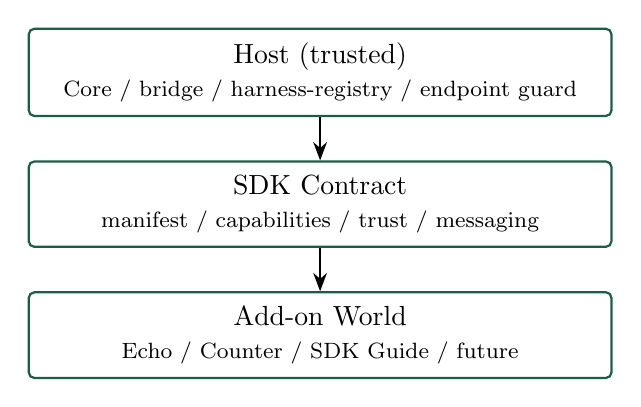
\begin{tikzpicture}[
  node distance=0.55cm,
  box/.style={draw=accent, thick, rounded corners=2pt, align=center,
              inner sep=5pt, minimum width=7.4cm},
  arrow/.style={-{Stealth}, thick}
]
  \node[box] (core) {Host (trusted) \\ \footnotesize Core / bridge / harness-registry / endpoint guard};
  \node[box, below=of core] (sdk) {SDK Contract \\ \footnotesize manifest / capabilities / trust / messaging};
  \node[box, below=of sdk] (addons) {Add-on World \\ \footnotesize Echo / Counter / SDK Guide / future};
  \draw[arrow] (core) -- (sdk);
  \draw[arrow] (sdk) -- (addons);
\end{tikzpicture}
\end{center}

The lifecycle a workspace add-on traverses is:

\begin{center}
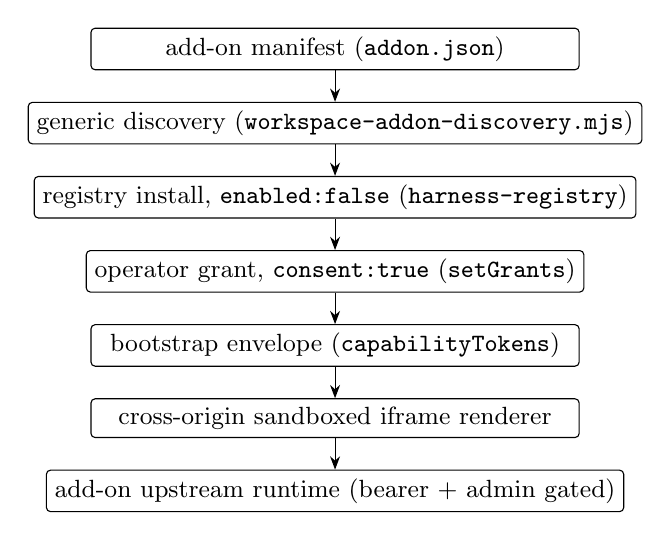
\begin{tikzpicture}[
  node distance=0.4cm,
  stage/.style={draw, rounded corners=1.5pt, align=center, inner sep=3pt,
                minimum width=6.2cm, font=\small},
  arrow/.style={-{Stealth}}
]
  \node[stage] (m) {add-on manifest (\texttt{addon.json})};
  \node[stage, below=of m] (d) {generic discovery (\texttt{workspace-addon-discovery.mjs})};
  \node[stage, below=of d] (r) {registry install, \texttt{enabled:false} (\texttt{harness-registry})};
  \node[stage, below=of r] (g) {operator grant, \texttt{consent:true} (\texttt{setGrants})};
  \node[stage, below=of g] (b) {bootstrap envelope (\texttt{capabilityTokens})};
  \node[stage, below=of b] (i) {cross-origin sandboxed iframe renderer};
  \node[stage, below=of i] (u) {add-on upstream runtime (bearer + admin gated)};
  \draw[arrow] (m) -- (d);
  \draw[arrow] (d) -- (r);
  \draw[arrow] (r) -- (g);
  \draw[arrow] (g) -- (b);
  \draw[arrow] (b) -- (i);
  \draw[arrow] (i) -- (u);
\end{tikzpicture}
\end{center}

\subsection{Authority}

The single grant authority is the existing \texttt{harness-registry}
(\texttt{createHarnessRegistry}), the same registry that already gates harness
adapter routes. Workspace add-ons were extended onto it \emph{without}
inventing a second registry:

\begin{itemize}[leftmargin=1.5em]
  \item \texttt{executeAddonsStatus} installs every discovered manifest with
        \texttt{enabled: false}.
  \item \texttt{POST /addons/workspace/grant} proxies
        \texttt{registry.setGrants(addonId, grants, \{ consent: true,
        expectedRevision \})}; \texttt{consent: false} throws
        \texttt{permission-denied} at the registry boundary.
  \item \texttt{POST /addons/workspace/bootstrap} returns
        \texttt{capabilityTokens[cap].token} only for capabilities the host has
        granted.
\end{itemize}

\subsection{Isolation and token delivery}

Add-ons render inside a sandboxed iframe whose \texttt{src} is the add-on's own
upstream origin (for example \url{http://127.0.0.1:47321}), using
\texttt{sandbox="allow-scripts allow-same-origin"}. Because the iframe is
same-origin with its own upstream and cross-origin from the extension, it can
call its own API without CORS yet cannot reach the extension's
\texttt{chrome.*} APIs, storage, or the bridge. No
\texttt{Access-Control-Allow-Origin} header is emitted by any upstream.

Capability tokens are delivered from the trusted extension to the iframe via
\texttt{postMessage} with \texttt{targetOrigin} pinned to the add-on's origin.
The add-on validates both \texttt{event.source} and the message type before
trusting it. The bridge token, the admin token, and any provider credential
never reach the add-on.

\section{The Reference Add-ons}

Three add-ons were built, all registered through the same generic mechanism
with zero Core changes:

\begin{center}
\begin{tabular}{@{}p{3.0cm}p{3.4cm}p{2.5cm}p{3.4cm}@{}}
\toprule
\textbf{Add-on} & \textbf{ID} & \textbf{Port} & \textbf{Purpose} \\
\midrule
Resonant Echo & \texttt{addon.resonant-echo} & 47321 & Deterministic echo; proves the bearer-gated round-trip \\
Resonant Counter & \texttt{addon.resonant-counter} & 47322 & Second add-on; proves the mechanism is generic \\
SDK Guide & \texttt{addon.sdk-guide} & 47323 & 9-step tutorial; teaches the SDK while using it \\
\bottomrule
\end{tabular}
\end{center}

\subsection{Resonant Echo}

A deterministic echo responder. Its mutating route \texttt{POST
/api/echo/message} is bearer-gated; it returns the message verbatim as
\texttt{Resonant Echo received: "<message>"}. It carries no model, provider, or
network dependency.

\subsection{Resonant Counter}

A deterministic stateful counter exposing \texttt{POST
/api/counter/\{increment,decrement,reset\}} and a public \texttt{GET
/api/counter/value}. State lives only in the upstream's memory; the host never
reads or writes it. Its existence is the \emph{replacement proof}: a second,
unrelated add-on onboards through the exact same mechanism with no additional
Core code.

\subsection{SDK Guide}

A tutorial add-on that walks the developer through discovery, manifest
validation, capability request, host consent, grant, sandboxed rendering, an
authorized call, a denied call, and revocation. Each step is a \emph{real} HTTP
outcome from the operator-started guide upstream --- step 7 reports \texttt{200},
step 8 reports \texttt{401} (wrong bearer), and step 9 reports \texttt{403}
(host-revoked). This is the strongest form of the replacement proof: an add-on
that teaches the SDK while itself being an SDK add-on.

\section{Capability and Security Model}

The public capability vocabulary is \texttt{ADDON\_CAPABILITIES} (14 entries):
\texttt{filesystem}, \texttt{archive-read}, \texttt{archive-intake-write},
\texttt{chat-interface}, \texttt{memory-provider}, \texttt{providers},
\texttt{shell}, \texttt{network}, \texttt{ui-embedding},
\texttt{browser-control}, \texttt{agent-delegation}, \texttt{agent-runtime},
\texttt{notifications}, and \texttt{device-integration}. The three reference
add-ons request only \texttt{network}, authored with \texttt{granted: false}.

Each grant is a \texttt{CapabilityGrant \{ capability, granted, scope,
revocationBehavior \}} with \texttt{CapabilityScope}
(\texttt{none|self|workspace|shared|system|intake-only}) and
\texttt{RevocationBehavior} (\texttt{hard-stop|degrade|hide-surface}).

The status-code contract is explicit and exercised end-to-end:

\begin{center}
\begin{tabular}{@{}p{4.6cm}p{7.6cm}@{}}
\toprule
\textbf{Status} & \textbf{Meaning} \\
\midrule
\texttt{200} & operation succeeded with a valid bearer \\
\texttt{401} & caller presented a missing or wrong bearer (audience-bound credential boundary) \\
\texttt{403} & host revoked the grant; the bearer is valid but policy is closed (real host-policy result) \\
\texttt{503} & upstream started without an operator-pinned bearer; no mutating call is authorized \\
\bottomrule
\end{tabular}
\end{center}

Two distinct operator-pinned tokens per add-on enforce the boundary:

\begin{itemize}[leftmargin=1.5em]
  \item \textbf{Bearer token} --- delivered to the iframe via the bootstrap
        envelope and carried as \texttt{Authorization: Bearer} on every
        mutating request. Held by the bridge; never in HTML or a URL.
  \item \textbf{Admin token} --- gates \texttt{POST /admin/deny} on the
        upstream. Never delivered to the iframe; the bridge uses it
        out-of-band to flip the upstream's in-memory deny flag.
\end{itemize}

Token comparison in the upstreams is a constant-time XOR compare; wrong,
case-shifted, and appended-byte tokens are rejected identically.

\section{How It Was Built}

The work was delivered in nine phases (P0--P9), each independently verified
before the next was authorized.

\begin{center}
\begin{tabular}{@{}p{3.2cm}p{9.0cm}@{}}
\toprule
\textbf{Phase} & \textbf{Delivered} \\
\midrule
P0 & baseline frozen on \texttt{upstream/dev @ 19665c06}; full gate recorded \\
P1 & architecture inventory; mapped 002 findings to current-\texttt{dev} disposition \\
P2 & scaffold + validating Echo manifest \\
P3 & Echo round-trip through the real extension \\
P4 & Counter add-on + cross-add-on isolation \\
P5 & sandboxed cross-origin renderer (\texttt{createWorkspaceAddonIframe}) \\
P6 & host-owned grants; 401/403 lifecycle; grant-wipe regression fixed \\
P7 & SDK Guide add-on (9-step tutorial with real policy denials) \\
P8 & adversarial red-team (11-attack matrix) + route-audit gap closed \\
P9 & live demo; README-only reproduction + walk-the-demo npm script \\
\bottomrule
\end{tabular}
\end{center}

\section{What Was Found}

The independent review loop surfaced and corrected a series of real defects
that the initial automated suite did not catch. These are recorded because they
explain \emph{why} the demonstration now works and why a browser-visible test
is a necessary gate.

\subsection{Resolved during the build}

\begin{center}
\begin{tabular}{@{}p{1.0cm}p{6.6cm}p{4.6cm}@{}}
\toprule
\textbf{ID} & \textbf{Finding} & \textbf{Resolution} \\
\midrule
R1 & Self-grant placeholder: bootstrap tokens were derived from author-controlled \texttt{grantPresets} (\texttt{granted: true}). & Closed in P6: grants sourced from \texttt{harness-registry}, never \texttt{grantPresets}. \\
R2 & CP4 false-green: the Counter live test reported 1/1 but failed on a stale \texttt{bridge-config.generated.js}. & Closed: stale-config cleanup added, matching Echo. \\
R3 & CP3 deferred the real-extension test and substituted a network smoke test. & Closed: \texttt{echo-extension-live.test.mjs} loads the real unpacked extension. \\
R4 & \texttt{apiBasePath} carried an origin rather than a path; a dead no-op loop remained. & Closed: field dropped, loop removed. \\
R5 & Grant-wipe on re-poll: re-running \texttt{registry.install()} on every \texttt{/addons/status} poll reset grants. & Closed: guarded install + regression test. \\
\bottomrule
\end{tabular}
\end{center}

\subsection{Verification-quality corrections}

Independent re-verification of the adversarial suite found several test titles
that overstated what each test alone proved (no security hole, but honest
labels matter). All were corrected and recorded as \texttt{V1}--\texttt{V6}:

\begin{itemize}[leftmargin=1.5em]
  \item The ``12 attacks'' claim was actually 11 rows; the open-mirror/proxy
        concern was made an explicit negative assertion (V1).
  \item The use-after-revoke test drives only the admin channel; the
        both-channel witness is the real-extension test (V2).
  \item The forged-\texttt{postMessage} tests are static shape checks, not
        runtime forgery tests (V3).
  \item The ``constant-time'' test asserts rejection, not a timing measurement
        (V4).
  \item The port-collision test's launcher-outcome value is now asserted, with
        the manifest-unchanged invariant stated honestly (V5).
  \item \texttt{runtime.command} is inert by construction (declarative
        discovery, no spawn path), now stated explicitly (V6).
\end{itemize}

\subsection{Deferred items (recorded, not lost)}

\begin{center}
\begin{tabular}{@{}p{1.0cm}p{11.2cm}@{}}
\toprule
\textbf{ID} & \textbf{Item} \\
\midrule
D1 & Host-mediated enforcement: the iframe still calls its own upstream directly, so the host is not the only path a mutating request can take. \\
D2 & Operator-pinned bearer tokens are static, not host-minted, expiring, audience-bound credentials. \\
D3 & Revocation is an out-of-band \texttt{/admin/deny} signal, not the host-mediated production shape. \\
D4 & Real-extension tests are not in the default CI run. \\
D5 & Pre-existing \texttt{openai-harness-adapter} timing flake, unrelated to the demo. \\
D6 & \texttt{harness-registry.install()} is non-idempotent (re-install resets grants). \\
\bottomrule
\end{tabular}
\end{center}

\section{Adversarial Red-Team}

The trust boundaries were red-teamed. Every attack fails safely; no attack is
``passed'' by weakening a control, and no mock bridge skips auth/CORS/origin
checks. The matrix covers the 12 red-team concerns from the checklist,
consolidated into 11 named attacks:

\begin{center}
\begin{tabular}{@{}p{0.9cm}p{3.6cm}p{7.7cm}@{}}
\toprule
\textbf{\#} & \textbf{Attack} & \textbf{Defensive control} \\
\midrule
1 & Secrets leak & bootstrap envelope carries only the host-minted bearer; no token in HTML/URL/env. \\
2 & Cross-add-on credential reuse & per-add-on audience-bound bearer; 3-way isolation. \\
3 & Use-after-revoke & two independent channels (registry + admin); bearer dead until both restored. \\
4 & Self-grant / outside-capabilities / no consent & registry \texttt{permission-denied} + optimistic concurrency. \\
5 & Forged \texttt{postMessage} & \texttt{event.source} and type checks; parent pins \texttt{targetOrigin}. \\
6 & Arbitrary entrypoint / non-loopback / non-local-service & discovery rejects; no spawn path. \\
7 & Open mirror/proxy route & explicit negative assertion: no \texttt{/addons/workspace/proxy*} route. \\
8 & Malformed credentials & strict constant-time compare; 503/401/200 distinction. \\
9 & Crash + bridge restart & durable registry journal preserves grants. \\
10 & Port collision & bridge never rewrites the manifest entrypoint. \\
11 & Hermes/OpenCode/Living Archive displacement & host services remain wired and capability-gated. \\
\bottomrule
\end{tabular}
\end{center}

\section{Test Results}

All suites are green on Node \texttt{v26.0.0} (the repository requires
\texttt{>=24.21.0}):

\begin{center}
\begin{tabular}{@{}p{8.6cm}p{4.6cm}@{}}
\toprule
\textbf{Suite} & \textbf{Result} \\
\midrule
\texttt{npx vitest run} & 721/721 \\
\texttt{npx vitest run --config examples/sdk-demo/vitest.config.ts} & 58/58 \\
\texttt{npm run test:browser-host} & 13/13 \\
\texttt{sd003-p8-adversarial.test.mjs} & 10/10 \\
\texttt{bridge-route-capability-audit.test.mjs} & 5/5 \\
\texttt{harness-registry-workspace-addon.test.mjs} & 8/8 \\
\texttt{addons-status-grant-regression.test.mjs} & 2/2 \\
\texttt{npm run test:sdk-demo:extension} (four live tests) & 4/4 \\
\midrule
\textbf{Total} & \textbf{821} \\
\bottomrule
\end{tabular}
\end{center}

The four real-extension tests are the strongest evidence: each boots its own
upstream and bridge, loads the actual unpacked extension in Chrome, and drives
the lifecycle against the real host boundary --- no \texttt{--disable-extensions},
no \texttt{Page.addScriptToEvaluateOnNewDocument}, no mock bridge that skips
auth.

\section{User Guide}

This section describes how to reproduce the demonstration from a clean
checkout.

\subsection{Prerequisites}

\begin{itemize}[leftmargin=1.5em]
  \item Node.js \texttt{>=24.21.0} (see \texttt{.nvmrc}; developed on
        \texttt{v26.0.0}).
  \item A Chromium-family browser (Chrome, Edge, Brave, Arc).
\end{itemize}

\subsection{Checkout and install}

\begin{lstlisting}[language=bash]
git clone https://github.com/vonstegen/2.0.0-alpha.git
cd 2.0.0-alpha
git checkout r-and-d/sdk-demo-003-current-dev
npm ci
\end{lstlisting}

\subsection{Start the three upstreams}

Open three terminals; the bridge never spawns them.

\begin{lstlisting}[language=bash]
node examples/sdk-demo/echo/server.mjs \
  --echo-bearer-token=demo-echo-bearer \
  --echo-admin-token=demo-echo-admin

node examples/sdk-demo/counter/server.mjs \
  --counter-bearer-token=demo-counter-bearer \
  --counter-admin-token=demo-counter-admin

node examples/sdk-demo/sdk-guide/server.mjs \
  --sdk-guide-bearer-token=demo-guide-bearer \
  --sdk-guide-admin-token=demo-guide-admin
\end{lstlisting}

\subsection{Start the bridge}

\begin{lstlisting}[language=bash]
node browser-first/host/run-bridge-minimal.mjs \
  --bridge-port=47300 \
  --bridge-token=demo-bridge-token \
  --capability-bootstrap-token=demo-bootstrap-token \
  --addon-runtime-read-token=demo-addon-runtime-read \
  --addon-runtime-control-token=demo-addon-runtime-control \
  --echo-bearer-token=demo-echo-bearer \
  --echo-admin-token=demo-echo-admin \
  --counter-bearer-token=demo-counter-bearer \
  --counter-admin-token=demo-counter-admin \
  --sdk-guide-bearer-token=demo-guide-bearer \
  --sdk-guide-admin-token=demo-guide-admin
\end{lstlisting}

\emph{(The full capability-token flag set is the
\texttt{BRIDGE\_CAPABILITY\_TOKEN\_SPECS} table in
\texttt{browser-first/host/bridge-capability-tokens.mjs}; the demo-relevant
subset above is sufficient.)}

\subsection{Load the extension}

\begin{enumerate}[leftmargin=1.5em]
  \item In Chrome, open \texttt{chrome://extensions}.
  \item Enable \textbf{Developer mode}.
  \item Choose \textbf{Load unpacked} and select
        \texttt{browser-first/resonantos-side-panel-extension}.
  \item Open the ResonantOS side panel and navigate to \textbf{Add-ons}.
\end{enumerate}

\subsection{Walk the lifecycle}

\begin{enumerate}[leftmargin=1.5em]
  \item \textbf{Open Resonant Echo}, type \texttt{Hello Manolo}, and press
        \textbf{SEND}; the response \texttt{Resonant Echo received: "Hello
        Manolo"} renders.
  \item \textbf{Grant} an add-on; the registry records the grant and the add-on
        can call its upstream (\texttt{200}).
  \item Present a \textbf{wrong bearer}; the upstream returns \texttt{401}.
  \item \textbf{Revoke}; the upstream returns \texttt{403} (real host policy).
  \item \textbf{Admin-revoke + re-grant}; the upstream returns \texttt{200}
        again.
  \item Switch to \textbf{Hermes}, \textbf{OpenCode}, and \textbf{Living
        Archive}; each remains present and capability-gated.
\end{enumerate}

\subsection{Run the test suite}

\begin{lstlisting}[language=bash]
npm run test:sdk-demo:vitest        # 58/58 deterministic
npm run test:sdk-demo:extension     # 4/4 real-browser
npx vitest run                      # 721/721
npm run test:browser-host           # 13/13
node --test --test-concurrency=1 browser-first/test/sd003-p8-adversarial.test.mjs
\end{lstlisting}

\section{Demo-vs-Production Honesty}

The demonstration is deliberately honest about what it does and does not prove.
The enforcement point in the demo is the \emph{add-on's own upstream}: a
bearer-gated mutating route plus an admin-gated in-memory deny flag, with the
bridge calling \texttt{/admin/deny} out-of-band. This is the cleanest mechanism
that fits an operator-started local-service add-on without inventing a second
host transport.

It proves: (a) the host-owned registry is the right authority; (b)
consent-gated grant and revoke round-trip through the registry; (c) the
per-add-on audience boundary holds; and (d) the upstream distinguishes
\texttt{401} (wrong bearer) from \texttt{403} (host-revoked).

It does \emph{not} prove: (e) the host is the \emph{only} path a mutating
request can take --- the iframe still has direct loopback access to its own
upstream. Closing (e) is the central item in the way forward.

\section{The Way Forward Toward a Running SDK Platform}

The demonstration is a verified boundary, not a finished product. The
following sequence turns it into a production running SDK platform.

\subsection{Close the enforcement gap (D1 + D3)}

Route the iframe's mutating requests through a bridge-owned proxy ---
\texttt{POST /addons/workspace/proxy/\allowbreak\{addonId\}/api/...} --- that is the
\emph{only} listener on the upstream's loopback port, validates the grant
before forwarding, and injects a host-side token. The iframe then has no direct
loopback path, so the host becomes the sole enforcement point, and revocation
collapses into ``stop forwarding'' at the bridge boundary rather than an
add-on-side flag.

\subsection{Token hygiene (D2)}

Replace the static operator-pinned bearer with host-minted, expiring,
audience-bound per-grant tokens, rotated on revoke. The harness-boundary
machinery already mints signed session references; workspace add-ons should
consume the same model rather than a shared static value.

\subsection{Registry idempotency (D6)}

Decide and implement \texttt{harness-registry.install()} semantics so an
identical re-install either no-ops or rejects, removing the latent footgun that
re-install resets grants.

\subsection{CI wiring (D4)}

Promote the four real-extension tests into the default gate with a
skip-when-no-browser policy, so the browser-visible lifecycle cannot silently
drop out of CI.

\subsection{Flake hygiene (D5)}

Re-verify \texttt{openai-harness-adapter.test.mjs} on the pinned Node 24.21.0
and fix or exclude it independently of the demo.

\subsection{Merge path}

After the P10 integration review (diff audit against \texttt{upstream/dev},
full 002-findings disposition, and PR notes), fast-forward the branch into the
canonical fork, then reconcile with \texttt{dev} --- no force-push, no push to
the ResonantOS org without review.

\subsection{Publish the SDK contract}

Publish \texttt{@resonantos/addon-sdk} to npm so add-on authors consume a
versioned, stable contract rather than a repository path. This is the
author-facing boundary that makes the demonstration a platform.

\subsection{Replace deterministic add-ons with a real provider}

Swap the deterministic Echo/Counter responders for a real provider-backed
add-on (the existing \texttt{openai-compatible-harness} reference manifest is
the pattern), reusing the same discovery/registry/bridge/extension socket. This
proves the boundary carries real work, not just a canned round-trip.

\section{Conclusion}

\textsc{SDK-DEMO-003} proves, in the real browser extension, that a
third-party-style add-on can be discovered, validated, registered, granted,
enforced, and revoked through a single generic contract with no
add-on-specific Core code and no parallel trust model. Three add-ons ---
Resonant Echo, Resonant Counter, and the SDK Guide --- onboard through the same
mechanism; grants are host-owned and consent-gated; a wrong credential returns
\texttt{401} and a revoked grant returns a real \texttt{403}; the iframe is
isolated; the adversarial matrix fails safe; and the full 821-test gate is
green. The remaining work --- host-mediated enforcement, token rotation,
CI wiring, and npm publication --- is enumerated, and the demonstration is
positioned as the verified boundary on which that production platform is built.

\end{document}
